\tikzstyle{int}=[draw=BlueIASS, fill=GreyIASS, minimum size=2em]
\newcommand{\drawarc}[5]{ %radius, start angle, end angle, node position, node text, arc x-coord, arc y-coord
    \ifnum#3<#2
        \draw[thick, #4] arc (#2:360:#1) arc (0:#3:#1);
        \node[#4] {#5};
    \else
        \draw[thick, #4] arc (#2:#3:#1);
        \node[#4] {#5};
    \fi
    \draw[black, thick, rounded corners=.2pt, #4] (#3:#1) -- (0,0) -- (#2:#1) ;
}
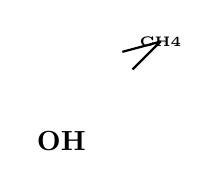
\begin{tikzpicture}[node distance=1.78cm,auto]
    \node (a) [align=center] {\textbf{OH}};
    %\node (b) [above right of = a, align=center] {\textbf{\tiny{\ce{CH4}}}};
    \drawarc{5mm}{225}{195}{above right of = a}{\textbf{\tiny{\ce{CH4}}}};
%    \node [int] (a) [align=center, fill=white]{\textbf{\LARGE{\ce{CH4}}}};
%    
%    \node [int] (b) [below right of = a, align=center]{\textbf{HCHO}};
%    \node [int] (c) [above of = a, align=center] {\textbf{\ce{HO2}}}; 
%    \node [int] (d) [below left of = a, align=center]{\textbf{\ce{CH3O2}}};
%    \node [int] (f) [left of = a, align=center]{\textbf{CO}};
%    \node [int] (g) [right of = a, align=center] {\textbf{\ce{OH}}};
%    
%    \path [->, draw=BlueIASS, fill=BlueIASS] (a) edge node {} (b);
%    \path [->, draw=BlueIASS, fill=BlueIASS] (a) edge node {} (c);
%    \path [->, draw=BlueIASS, fill=BlueIASS] (a) edge node {} (d);
%    \path [->, draw=BlueIASS, fill=BlueIASS] (a) edge node {} (f);
%    \path [->, draw=BlueIASS, fill=BlueIASS] (a) edge node {} (g);
%
%    \node [text=BlueIASS] (h) [below = 1mm of d, align=center] {\footnotesize{\textbf{CH3O2\_CH4}}};
%    \node [text=BlueIASS] (i) [below = 1mm of b, align=center] {\footnotesize{\textbf{HCHO\_CH4}}};
%    \node [text=BlueIASS] (j) [above = 0.5mm of f, align=center] {\footnotesize{\textbf{CO\_CH4}}};
\end{tikzpicture}
